\documentclass{article}
\input ../Resources/latex/std-macros
\usepackage{times}
\usepackage{xspace}
\usepackage[usenames,dvipsnames]{color}
\usepackage{booktabs}
\usepackage{colortbl}
\usepackage{uist}
\usepackage{amsmath}
\usepackage{graphicx}


\newcommand{\system}{Colorific\xspace}
\newcommand{\graycol}{\cellcolor[gray]{0.7}}

\begin{document}

% --- Copyright notice ---
\conferenceinfo{UIST'09}{October 4-7, 2009, Victoria, British Columbia, Canada}
\CopyrightYear{2009}
\crdata{978-1-60558-745-5/09/10}

% Uncomment the following line to hide the copyright notice
 \toappear{}
% ------------------------


\title{\system: A Mixed Initiative Model for \\Choosing the Right Color}

%%
%% Note on formatting authors at different institutions, as shown below:
%% Change width arg (currently 7cm) to parbox commands as needed to
%% accommodate widest lines, taking care not to overflow the 17.8cm line width.
%% Add or delete parboxes for additional authors at different institutions. 
%% If additional authors won't fit in one row, you can add a "\\"  at the
%% end of a parbox's closing "}" to have the next parbox start a new row.
%% Be sure NOT to put any blank lines between parbox commands!
%%

\author{
\parbox[t]{9cm}{\centering
	     {\em Chinmay Kulkarni}\\
	     Stanford University HCI Group\\
              Computer Science Department\\
	     Stanford, CA 94305\\
	     chinmay@cs.stanford.edu}
\parbox[t]{9cm}{\centering
	     {\em Julie Fortuna}\\
	     Stanford University HCI Group\\
              Computer Science Department\\
	     Stanford, CA 94305\\
	     jfortuna@stanford.edu}
}

\maketitle

\abstract
Is it possible to automatically create a color palette relevant to a topic? Could such a palette be used to guide color choices while visualizing data? We envision a tool that automatically creates aesthetically pleasing and topic-relevant palettes for a  large class of topics. In order to do this, we must first extract palettes from color pixel values of images from Google Images via clustering and topic models. 

\classification{H5.2 [Information interfaces and presentation]:
User Interfaces. - Graphical user interfaces.}

\terms{Design, Human Factors, Experimentation}

\keywords{Information visualization, colors, crowdsourcing, user study, mixed initiative}

\tolerance=400 
  % makes some lines with lots of white space, but 	
  % tends to prevent words from sticking out in the margin

\section{INTRODUCTION}
\input introduction.tex

\section{RELATED WORK}
\input related.tex
\section{SYSTEM DESCRIPTION}
\input algorithm.tex
\section{SYSTEM EVALUATION}
\input evaluation.tex
\section{DISCUSSION}
\input discussion.tex
\section{DESIGNING WITH COLORIFIC}
\subsection{Scenario}
\system is designed to help novices with little experience in designing information visualizations quickly choose appropriate and compelling colors for their visualizations. Let's examine David, a football fan, as he makes a bar chart of the number of games won by a selection of Pac-10 football teams. 

David begins making his chart in Microsoft Excel, but Excel has automatically colored each bar from a pre-defined set of colors. David wants to color each bar a representative color for the team. However, both the Cal Bears and the UCLA Bruins have the colors blue and gold. Which should be blue, and which should be gold? He loads \system to find out. David enters the specific topics he is plotting, such as the Stanford Cardinal and the Cal Bears, as well as their values. \system plots his values on a bar chart and automatically generates a selection of four potential palettes he can choose from. David selects one automatically generated palette, which looks almost the way he wants it. However, after seeing the results in context, he thinks the Cal Bears bar should be gold instead of blue. He clicks on the bar and is presented with a selection of other \system generated colors for the Cal Bears, as well as a color picker that allows him to tweak \system colors or select his own. 

\begin{center}
\scalebox{0.25}{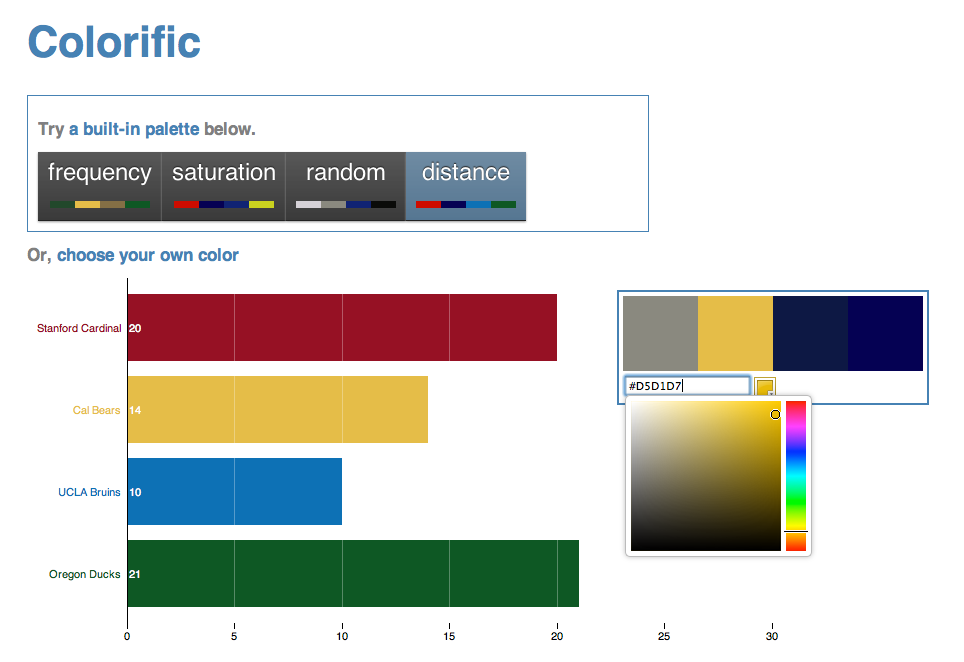
\includegraphics{colorific_screenshot.png}}
\end{center}

\subsection{Pilot Feedback}
pilot blah

\section{DESIGN SPACE}
\system provides one point in the space of many data visualization tools. We summarize the decisions we made using the design space in \ref{design-space}. This representation of the design space is not meant to be exhaustive, but merely informative. 

\begin{figure}
\label{design-space}
\scalebox{0.75}{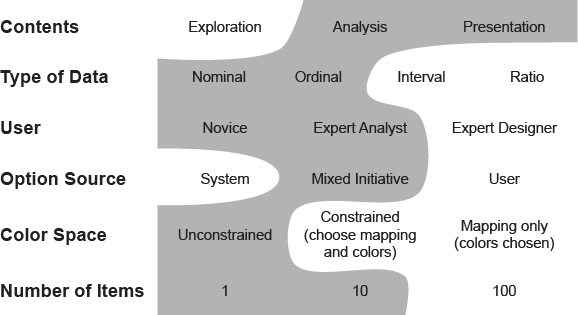
\includegraphics{design_space.png}}
\caption{\system Design space. Implemented choices in gray.}
\end{figure}
\Subsection{design-context}{Design Context} We believe having the right colors for a visualization help most in the analysis and the presentation stages. Therefore, \system provides no support for the ETL (extract-transform-load) stage of data visualization. However, these stages may also benefit, and perhaps guide the analyst in deciding which data is interesting. In the future, it would also be beneficial to incorporate \system into a larger data visualization tool so people can change visualization colors in context of their data.

\Subsection{design-user}{User} \system is meant for non-expert users and possibly expert analysts. 
 For novices, the main advantage of \system are pre-made palettes, which already have desirable properties, but can be tweaked and edited. For experts, \system's main advantage is saving time. While the expert designer could  benefit from such a system, designers use more advanced tools and often develop their own methods for extracting colors from images.
 
\Subsection{color-space}{Color Space} \system assumes that any color from the LAB space is an equally viable candidate. This may not be the case where the color space is constrained (for example, in printing techniques where only a few colors are available). While our method can be extended to these applications, by constraining the clustering algorithm,  we defer it to future work.

\Subsection{number-items}{Number of Items} Since \system is a mixed initiative system, user input is still required for choosing the final colors. This makes it unwieldy where hundreds of items are involved. However, a visualization with hundreds of nominal variables is probably ill-designed to begin with, and perhaps no system can find colors that are adequately separated.

\section{CONCLUSION}
CEK Make up stuff

\section{ACKNOWLEDGMENTS} 
CEK Thank Jeff, Scott and Jesse.
(BOTH together 150 words)


\bibliographystyle{abbrv}

\bibliography{../Resources/references/color-refs,../Resources/references/recommender-refs}
\end{document}
